
% Default to the notebook output style

    


% Inherit from the specified cell style.




    
\documentclass[11pt]{article}

    
    
    \usepackage[T1]{fontenc}
    % Nicer default font (+ math font) than Computer Modern for most use cases
    \usepackage{mathpazo}

    % Basic figure setup, for now with no caption control since it's done
    % automatically by Pandoc (which extracts ![](path) syntax from Markdown).
    \usepackage{graphicx}
    % We will generate all images so they have a width \maxwidth. This means
    % that they will get their normal width if they fit onto the page, but
    % are scaled down if they would overflow the margins.
    \makeatletter
    \def\maxwidth{\ifdim\Gin@nat@width>\linewidth\linewidth
    \else\Gin@nat@width\fi}
    \makeatother
    \let\Oldincludegraphics\includegraphics
    % Set max figure width to be 80% of text width, for now hardcoded.
    \renewcommand{\includegraphics}[1]{\Oldincludegraphics[width=.8\maxwidth]{#1}}
    % Ensure that by default, figures have no caption (until we provide a
    % proper Figure object with a Caption API and a way to capture that
    % in the conversion process - todo).
    \usepackage{caption}
    \DeclareCaptionLabelFormat{nolabel}{}
    \captionsetup{labelformat=nolabel}

    \usepackage{adjustbox} % Used to constrain images to a maximum size 
    \usepackage{xcolor} % Allow colors to be defined
    \usepackage{enumerate} % Needed for markdown enumerations to work
    \usepackage{geometry} % Used to adjust the document margins
    \usepackage{amsmath} % Equations
    \usepackage{amssymb} % Equations
    \usepackage{textcomp} % defines textquotesingle
    % Hack from http://tex.stackexchange.com/a/47451/13684:
    \AtBeginDocument{%
        \def\PYZsq{\textquotesingle}% Upright quotes in Pygmentized code
    }
    \usepackage{upquote} % Upright quotes for verbatim code
    \usepackage{eurosym} % defines \euro
    \usepackage[mathletters]{ucs} % Extended unicode (utf-8) support
    \usepackage[utf8x]{inputenc} % Allow utf-8 characters in the tex document
    \usepackage{fancyvrb} % verbatim replacement that allows latex
    \usepackage{grffile} % extends the file name processing of package graphics 
                         % to support a larger range 
    % The hyperref package gives us a pdf with properly built
    % internal navigation ('pdf bookmarks' for the table of contents,
    % internal cross-reference links, web links for URLs, etc.)
    \usepackage{hyperref}
    \usepackage{longtable} % longtable support required by pandoc >1.10
    \usepackage{booktabs}  % table support for pandoc > 1.12.2
    \usepackage[inline]{enumitem} % IRkernel/repr support (it uses the enumerate* environment)
    \usepackage[normalem]{ulem} % ulem is needed to support strikethroughs (\sout)
                                % normalem makes italics be italics, not underlines
    

    
    
    % Colors for the hyperref package
    \definecolor{urlcolor}{rgb}{0,.145,.698}
    \definecolor{linkcolor}{rgb}{.71,0.21,0.01}
    \definecolor{citecolor}{rgb}{.12,.54,.11}

    % ANSI colors
    \definecolor{ansi-black}{HTML}{3E424D}
    \definecolor{ansi-black-intense}{HTML}{282C36}
    \definecolor{ansi-red}{HTML}{E75C58}
    \definecolor{ansi-red-intense}{HTML}{B22B31}
    \definecolor{ansi-green}{HTML}{00A250}
    \definecolor{ansi-green-intense}{HTML}{007427}
    \definecolor{ansi-yellow}{HTML}{DDB62B}
    \definecolor{ansi-yellow-intense}{HTML}{B27D12}
    \definecolor{ansi-blue}{HTML}{208FFB}
    \definecolor{ansi-blue-intense}{HTML}{0065CA}
    \definecolor{ansi-magenta}{HTML}{D160C4}
    \definecolor{ansi-magenta-intense}{HTML}{A03196}
    \definecolor{ansi-cyan}{HTML}{60C6C8}
    \definecolor{ansi-cyan-intense}{HTML}{258F8F}
    \definecolor{ansi-white}{HTML}{C5C1B4}
    \definecolor{ansi-white-intense}{HTML}{A1A6B2}

    % commands and environments needed by pandoc snippets
    % extracted from the output of `pandoc -s`
    \providecommand{\tightlist}{%
      \setlength{\itemsep}{0pt}\setlength{\parskip}{0pt}}
    \DefineVerbatimEnvironment{Highlighting}{Verbatim}{commandchars=\\\{\}}
    % Add ',fontsize=\small' for more characters per line
    \newenvironment{Shaded}{}{}
    \newcommand{\KeywordTok}[1]{\textcolor[rgb]{0.00,0.44,0.13}{\textbf{{#1}}}}
    \newcommand{\DataTypeTok}[1]{\textcolor[rgb]{0.56,0.13,0.00}{{#1}}}
    \newcommand{\DecValTok}[1]{\textcolor[rgb]{0.25,0.63,0.44}{{#1}}}
    \newcommand{\BaseNTok}[1]{\textcolor[rgb]{0.25,0.63,0.44}{{#1}}}
    \newcommand{\FloatTok}[1]{\textcolor[rgb]{0.25,0.63,0.44}{{#1}}}
    \newcommand{\CharTok}[1]{\textcolor[rgb]{0.25,0.44,0.63}{{#1}}}
    \newcommand{\StringTok}[1]{\textcolor[rgb]{0.25,0.44,0.63}{{#1}}}
    \newcommand{\CommentTok}[1]{\textcolor[rgb]{0.38,0.63,0.69}{\textit{{#1}}}}
    \newcommand{\OtherTok}[1]{\textcolor[rgb]{0.00,0.44,0.13}{{#1}}}
    \newcommand{\AlertTok}[1]{\textcolor[rgb]{1.00,0.00,0.00}{\textbf{{#1}}}}
    \newcommand{\FunctionTok}[1]{\textcolor[rgb]{0.02,0.16,0.49}{{#1}}}
    \newcommand{\RegionMarkerTok}[1]{{#1}}
    \newcommand{\ErrorTok}[1]{\textcolor[rgb]{1.00,0.00,0.00}{\textbf{{#1}}}}
    \newcommand{\NormalTok}[1]{{#1}}
    
    % Additional commands for more recent versions of Pandoc
    \newcommand{\ConstantTok}[1]{\textcolor[rgb]{0.53,0.00,0.00}{{#1}}}
    \newcommand{\SpecialCharTok}[1]{\textcolor[rgb]{0.25,0.44,0.63}{{#1}}}
    \newcommand{\VerbatimStringTok}[1]{\textcolor[rgb]{0.25,0.44,0.63}{{#1}}}
    \newcommand{\SpecialStringTok}[1]{\textcolor[rgb]{0.73,0.40,0.53}{{#1}}}
    \newcommand{\ImportTok}[1]{{#1}}
    \newcommand{\DocumentationTok}[1]{\textcolor[rgb]{0.73,0.13,0.13}{\textit{{#1}}}}
    \newcommand{\AnnotationTok}[1]{\textcolor[rgb]{0.38,0.63,0.69}{\textbf{\textit{{#1}}}}}
    \newcommand{\CommentVarTok}[1]{\textcolor[rgb]{0.38,0.63,0.69}{\textbf{\textit{{#1}}}}}
    \newcommand{\VariableTok}[1]{\textcolor[rgb]{0.10,0.09,0.49}{{#1}}}
    \newcommand{\ControlFlowTok}[1]{\textcolor[rgb]{0.00,0.44,0.13}{\textbf{{#1}}}}
    \newcommand{\OperatorTok}[1]{\textcolor[rgb]{0.40,0.40,0.40}{{#1}}}
    \newcommand{\BuiltInTok}[1]{{#1}}
    \newcommand{\ExtensionTok}[1]{{#1}}
    \newcommand{\PreprocessorTok}[1]{\textcolor[rgb]{0.74,0.48,0.00}{{#1}}}
    \newcommand{\AttributeTok}[1]{\textcolor[rgb]{0.49,0.56,0.16}{{#1}}}
    \newcommand{\InformationTok}[1]{\textcolor[rgb]{0.38,0.63,0.69}{\textbf{\textit{{#1}}}}}
    \newcommand{\WarningTok}[1]{\textcolor[rgb]{0.38,0.63,0.69}{\textbf{\textit{{#1}}}}}
    
    
    % Define a nice break command that doesn't care if a line doesn't already
    % exist.
    \def\br{\hspace*{\fill} \\* }
    % Math Jax compatability definitions
    \def\gt{>}
    \def\lt{<}
    % Document parameters
    \title{Quest2}
    
    
    

    % Pygments definitions
    
\makeatletter
\def\PY@reset{\let\PY@it=\relax \let\PY@bf=\relax%
    \let\PY@ul=\relax \let\PY@tc=\relax%
    \let\PY@bc=\relax \let\PY@ff=\relax}
\def\PY@tok#1{\csname PY@tok@#1\endcsname}
\def\PY@toks#1+{\ifx\relax#1\empty\else%
    \PY@tok{#1}\expandafter\PY@toks\fi}
\def\PY@do#1{\PY@bc{\PY@tc{\PY@ul{%
    \PY@it{\PY@bf{\PY@ff{#1}}}}}}}
\def\PY#1#2{\PY@reset\PY@toks#1+\relax+\PY@do{#2}}

\expandafter\def\csname PY@tok@w\endcsname{\def\PY@tc##1{\textcolor[rgb]{0.73,0.73,0.73}{##1}}}
\expandafter\def\csname PY@tok@c\endcsname{\let\PY@it=\textit\def\PY@tc##1{\textcolor[rgb]{0.25,0.50,0.50}{##1}}}
\expandafter\def\csname PY@tok@cp\endcsname{\def\PY@tc##1{\textcolor[rgb]{0.74,0.48,0.00}{##1}}}
\expandafter\def\csname PY@tok@k\endcsname{\let\PY@bf=\textbf\def\PY@tc##1{\textcolor[rgb]{0.00,0.50,0.00}{##1}}}
\expandafter\def\csname PY@tok@kp\endcsname{\def\PY@tc##1{\textcolor[rgb]{0.00,0.50,0.00}{##1}}}
\expandafter\def\csname PY@tok@kt\endcsname{\def\PY@tc##1{\textcolor[rgb]{0.69,0.00,0.25}{##1}}}
\expandafter\def\csname PY@tok@o\endcsname{\def\PY@tc##1{\textcolor[rgb]{0.40,0.40,0.40}{##1}}}
\expandafter\def\csname PY@tok@ow\endcsname{\let\PY@bf=\textbf\def\PY@tc##1{\textcolor[rgb]{0.67,0.13,1.00}{##1}}}
\expandafter\def\csname PY@tok@nb\endcsname{\def\PY@tc##1{\textcolor[rgb]{0.00,0.50,0.00}{##1}}}
\expandafter\def\csname PY@tok@nf\endcsname{\def\PY@tc##1{\textcolor[rgb]{0.00,0.00,1.00}{##1}}}
\expandafter\def\csname PY@tok@nc\endcsname{\let\PY@bf=\textbf\def\PY@tc##1{\textcolor[rgb]{0.00,0.00,1.00}{##1}}}
\expandafter\def\csname PY@tok@nn\endcsname{\let\PY@bf=\textbf\def\PY@tc##1{\textcolor[rgb]{0.00,0.00,1.00}{##1}}}
\expandafter\def\csname PY@tok@ne\endcsname{\let\PY@bf=\textbf\def\PY@tc##1{\textcolor[rgb]{0.82,0.25,0.23}{##1}}}
\expandafter\def\csname PY@tok@nv\endcsname{\def\PY@tc##1{\textcolor[rgb]{0.10,0.09,0.49}{##1}}}
\expandafter\def\csname PY@tok@no\endcsname{\def\PY@tc##1{\textcolor[rgb]{0.53,0.00,0.00}{##1}}}
\expandafter\def\csname PY@tok@nl\endcsname{\def\PY@tc##1{\textcolor[rgb]{0.63,0.63,0.00}{##1}}}
\expandafter\def\csname PY@tok@ni\endcsname{\let\PY@bf=\textbf\def\PY@tc##1{\textcolor[rgb]{0.60,0.60,0.60}{##1}}}
\expandafter\def\csname PY@tok@na\endcsname{\def\PY@tc##1{\textcolor[rgb]{0.49,0.56,0.16}{##1}}}
\expandafter\def\csname PY@tok@nt\endcsname{\let\PY@bf=\textbf\def\PY@tc##1{\textcolor[rgb]{0.00,0.50,0.00}{##1}}}
\expandafter\def\csname PY@tok@nd\endcsname{\def\PY@tc##1{\textcolor[rgb]{0.67,0.13,1.00}{##1}}}
\expandafter\def\csname PY@tok@s\endcsname{\def\PY@tc##1{\textcolor[rgb]{0.73,0.13,0.13}{##1}}}
\expandafter\def\csname PY@tok@sd\endcsname{\let\PY@it=\textit\def\PY@tc##1{\textcolor[rgb]{0.73,0.13,0.13}{##1}}}
\expandafter\def\csname PY@tok@si\endcsname{\let\PY@bf=\textbf\def\PY@tc##1{\textcolor[rgb]{0.73,0.40,0.53}{##1}}}
\expandafter\def\csname PY@tok@se\endcsname{\let\PY@bf=\textbf\def\PY@tc##1{\textcolor[rgb]{0.73,0.40,0.13}{##1}}}
\expandafter\def\csname PY@tok@sr\endcsname{\def\PY@tc##1{\textcolor[rgb]{0.73,0.40,0.53}{##1}}}
\expandafter\def\csname PY@tok@ss\endcsname{\def\PY@tc##1{\textcolor[rgb]{0.10,0.09,0.49}{##1}}}
\expandafter\def\csname PY@tok@sx\endcsname{\def\PY@tc##1{\textcolor[rgb]{0.00,0.50,0.00}{##1}}}
\expandafter\def\csname PY@tok@m\endcsname{\def\PY@tc##1{\textcolor[rgb]{0.40,0.40,0.40}{##1}}}
\expandafter\def\csname PY@tok@gh\endcsname{\let\PY@bf=\textbf\def\PY@tc##1{\textcolor[rgb]{0.00,0.00,0.50}{##1}}}
\expandafter\def\csname PY@tok@gu\endcsname{\let\PY@bf=\textbf\def\PY@tc##1{\textcolor[rgb]{0.50,0.00,0.50}{##1}}}
\expandafter\def\csname PY@tok@gd\endcsname{\def\PY@tc##1{\textcolor[rgb]{0.63,0.00,0.00}{##1}}}
\expandafter\def\csname PY@tok@gi\endcsname{\def\PY@tc##1{\textcolor[rgb]{0.00,0.63,0.00}{##1}}}
\expandafter\def\csname PY@tok@gr\endcsname{\def\PY@tc##1{\textcolor[rgb]{1.00,0.00,0.00}{##1}}}
\expandafter\def\csname PY@tok@ge\endcsname{\let\PY@it=\textit}
\expandafter\def\csname PY@tok@gs\endcsname{\let\PY@bf=\textbf}
\expandafter\def\csname PY@tok@gp\endcsname{\let\PY@bf=\textbf\def\PY@tc##1{\textcolor[rgb]{0.00,0.00,0.50}{##1}}}
\expandafter\def\csname PY@tok@go\endcsname{\def\PY@tc##1{\textcolor[rgb]{0.53,0.53,0.53}{##1}}}
\expandafter\def\csname PY@tok@gt\endcsname{\def\PY@tc##1{\textcolor[rgb]{0.00,0.27,0.87}{##1}}}
\expandafter\def\csname PY@tok@err\endcsname{\def\PY@bc##1{\setlength{\fboxsep}{0pt}\fcolorbox[rgb]{1.00,0.00,0.00}{1,1,1}{\strut ##1}}}
\expandafter\def\csname PY@tok@kc\endcsname{\let\PY@bf=\textbf\def\PY@tc##1{\textcolor[rgb]{0.00,0.50,0.00}{##1}}}
\expandafter\def\csname PY@tok@kd\endcsname{\let\PY@bf=\textbf\def\PY@tc##1{\textcolor[rgb]{0.00,0.50,0.00}{##1}}}
\expandafter\def\csname PY@tok@kn\endcsname{\let\PY@bf=\textbf\def\PY@tc##1{\textcolor[rgb]{0.00,0.50,0.00}{##1}}}
\expandafter\def\csname PY@tok@kr\endcsname{\let\PY@bf=\textbf\def\PY@tc##1{\textcolor[rgb]{0.00,0.50,0.00}{##1}}}
\expandafter\def\csname PY@tok@bp\endcsname{\def\PY@tc##1{\textcolor[rgb]{0.00,0.50,0.00}{##1}}}
\expandafter\def\csname PY@tok@fm\endcsname{\def\PY@tc##1{\textcolor[rgb]{0.00,0.00,1.00}{##1}}}
\expandafter\def\csname PY@tok@vc\endcsname{\def\PY@tc##1{\textcolor[rgb]{0.10,0.09,0.49}{##1}}}
\expandafter\def\csname PY@tok@vg\endcsname{\def\PY@tc##1{\textcolor[rgb]{0.10,0.09,0.49}{##1}}}
\expandafter\def\csname PY@tok@vi\endcsname{\def\PY@tc##1{\textcolor[rgb]{0.10,0.09,0.49}{##1}}}
\expandafter\def\csname PY@tok@vm\endcsname{\def\PY@tc##1{\textcolor[rgb]{0.10,0.09,0.49}{##1}}}
\expandafter\def\csname PY@tok@sa\endcsname{\def\PY@tc##1{\textcolor[rgb]{0.73,0.13,0.13}{##1}}}
\expandafter\def\csname PY@tok@sb\endcsname{\def\PY@tc##1{\textcolor[rgb]{0.73,0.13,0.13}{##1}}}
\expandafter\def\csname PY@tok@sc\endcsname{\def\PY@tc##1{\textcolor[rgb]{0.73,0.13,0.13}{##1}}}
\expandafter\def\csname PY@tok@dl\endcsname{\def\PY@tc##1{\textcolor[rgb]{0.73,0.13,0.13}{##1}}}
\expandafter\def\csname PY@tok@s2\endcsname{\def\PY@tc##1{\textcolor[rgb]{0.73,0.13,0.13}{##1}}}
\expandafter\def\csname PY@tok@sh\endcsname{\def\PY@tc##1{\textcolor[rgb]{0.73,0.13,0.13}{##1}}}
\expandafter\def\csname PY@tok@s1\endcsname{\def\PY@tc##1{\textcolor[rgb]{0.73,0.13,0.13}{##1}}}
\expandafter\def\csname PY@tok@mb\endcsname{\def\PY@tc##1{\textcolor[rgb]{0.40,0.40,0.40}{##1}}}
\expandafter\def\csname PY@tok@mf\endcsname{\def\PY@tc##1{\textcolor[rgb]{0.40,0.40,0.40}{##1}}}
\expandafter\def\csname PY@tok@mh\endcsname{\def\PY@tc##1{\textcolor[rgb]{0.40,0.40,0.40}{##1}}}
\expandafter\def\csname PY@tok@mi\endcsname{\def\PY@tc##1{\textcolor[rgb]{0.40,0.40,0.40}{##1}}}
\expandafter\def\csname PY@tok@il\endcsname{\def\PY@tc##1{\textcolor[rgb]{0.40,0.40,0.40}{##1}}}
\expandafter\def\csname PY@tok@mo\endcsname{\def\PY@tc##1{\textcolor[rgb]{0.40,0.40,0.40}{##1}}}
\expandafter\def\csname PY@tok@ch\endcsname{\let\PY@it=\textit\def\PY@tc##1{\textcolor[rgb]{0.25,0.50,0.50}{##1}}}
\expandafter\def\csname PY@tok@cm\endcsname{\let\PY@it=\textit\def\PY@tc##1{\textcolor[rgb]{0.25,0.50,0.50}{##1}}}
\expandafter\def\csname PY@tok@cpf\endcsname{\let\PY@it=\textit\def\PY@tc##1{\textcolor[rgb]{0.25,0.50,0.50}{##1}}}
\expandafter\def\csname PY@tok@c1\endcsname{\let\PY@it=\textit\def\PY@tc##1{\textcolor[rgb]{0.25,0.50,0.50}{##1}}}
\expandafter\def\csname PY@tok@cs\endcsname{\let\PY@it=\textit\def\PY@tc##1{\textcolor[rgb]{0.25,0.50,0.50}{##1}}}

\def\PYZbs{\char`\\}
\def\PYZus{\char`\_}
\def\PYZob{\char`\{}
\def\PYZcb{\char`\}}
\def\PYZca{\char`\^}
\def\PYZam{\char`\&}
\def\PYZlt{\char`\<}
\def\PYZgt{\char`\>}
\def\PYZsh{\char`\#}
\def\PYZpc{\char`\%}
\def\PYZdl{\char`\$}
\def\PYZhy{\char`\-}
\def\PYZsq{\char`\'}
\def\PYZdq{\char`\"}
\def\PYZti{\char`\~}
% for compatibility with earlier versions
\def\PYZat{@}
\def\PYZlb{[}
\def\PYZrb{]}
\makeatother


    % Exact colors from NB
    \definecolor{incolor}{rgb}{0.0, 0.0, 0.5}
    \definecolor{outcolor}{rgb}{0.545, 0.0, 0.0}



    
    % Prevent overflowing lines due to hard-to-break entities
    \sloppy 
    % Setup hyperref package
    \hypersetup{
      breaklinks=true,  % so long urls are correctly broken across lines
      colorlinks=true,
      urlcolor=urlcolor,
      linkcolor=linkcolor,
      citecolor=citecolor,
      }
    % Slightly bigger margins than the latex defaults
    
    \geometry{verbose,tmargin=1in,bmargin=1in,lmargin=1in,rmargin=1in}
    
    

    \begin{document}
    
    
    \maketitle
    
    

    
    \section{Quest 2: Regex, Files, Urls}\label{quest-2-regex-files-urls}

\textbf{STUDENT\_ID} = "35460312"\\
\textbf{QUEST\_NAME} = "QUEST2"\\
\textbf{CODING\_NAME} = "MonsterPeach"

    \begin{Verbatim}[commandchars=\\\{\}]
{\color{incolor}In [{\color{incolor}1}]:} \PY{c+c1}{\PYZsh{}Quest: Regex, Files, Urls}
        
        \PY{k+kn}{import} \PY{n+nn}{re}\PY{o}{,} \PY{n+nn}{pytest}\PY{o}{,} \PY{n+nn}{requests}
        
        
        \PY{n}{\PYZus{}\PYZus{}STUDENT\PYZus{}ID\PYZus{}\PYZus{}}  \PY{o}{=} \PY{l+s+s2}{\PYZdq{}}\PY{l+s+s2}{35460312}\PY{l+s+s2}{\PYZdq{}}        \PY{c+c1}{\PYZsh{} replace with your 8 digit student id}
        \PY{n}{\PYZus{}\PYZus{}QUEST\PYZus{}NAME\PYZus{}\PYZus{}} \PY{o}{=} \PY{l+s+s2}{\PYZdq{}}\PY{l+s+s2}{QUEST2}\PY{l+s+s2}{\PYZdq{}}           \PY{c+c1}{\PYZsh{} QUEST NAME}
        \PY{n}{\PYZus{}\PYZus{}CODING\PYZus{}NAME\PYZus{}\PYZus{}} \PY{o}{=} \PY{l+s+s2}{\PYZdq{}}\PY{l+s+s2}{MonsterPeach}\PY{l+s+s2}{\PYZdq{}}           \PY{c+c1}{\PYZsh{} replace with your coding name \PYZhy{} max 15 characters}
\end{Verbatim}


    \begin{Verbatim}[commandchars=\\\{\}]
{\color{incolor}In [{\color{incolor}2}]:} \PY{k}{def} \PY{n+nf}{count\PYZus{}vowels}\PY{p}{(}\PY{n}{mystr}\PY{p}{)}\PY{p}{:}
            \PY{l+s+sd}{\PYZdq{}\PYZdq{}\PYZdq{}return the number of vowels, upper and lowercase a,e,i,o,u in the string}
        \PY{l+s+sd}{    \PYZgt{}\PYZgt{}\PYZgt{} count\PYZus{}vowels(\PYZsq{}aaacvemmikkOOzzuU\PYZsq{})  \PYZhy{}\PYZgt{} 9}
        \PY{l+s+sd}{    \PYZdq{}\PYZdq{}\PYZdq{}}
            
            \PY{n}{mystr} \PY{o}{=} \PY{n}{mystr}\PY{o}{.}\PY{n}{lower}\PY{p}{(}\PY{p}{)}
            \PY{n}{vowel\PYZus{}list} \PY{o}{=} \PY{n}{re}\PY{o}{.}\PY{n}{findall}\PY{p}{(}\PY{l+s+sa}{r}\PY{l+s+s1}{\PYZsq{}}\PY{l+s+s1}{[aiueo]}\PY{l+s+s1}{\PYZsq{}}\PY{p}{,} \PY{n}{mystr}\PY{p}{)}    
            \PY{k}{return} \PY{n+nb}{len}\PY{p}{(}\PY{n}{vowel\PYZus{}list}\PY{p}{)}
\end{Verbatim}


    \begin{Verbatim}[commandchars=\\\{\}]
{\color{incolor}In [{\color{incolor}3}]:} \PY{n}{count\PYZus{}vowels}\PY{p}{(}\PY{l+s+s1}{\PYZsq{}}\PY{l+s+s1}{aaacvemmikkOOzzuU}\PY{l+s+s1}{\PYZsq{}}\PY{p}{)}
\end{Verbatim}


\begin{Verbatim}[commandchars=\\\{\}]
{\color{outcolor}Out[{\color{outcolor}3}]:} 9
\end{Verbatim}
            
    \begin{Verbatim}[commandchars=\\\{\}]
{\color{incolor}In [{\color{incolor}4}]:} \PY{k}{def} \PY{n+nf}{is\PYZus{}valid\PYZus{}python\PYZus{}hex}\PY{p}{(}\PY{n}{mystr}\PY{p}{)}\PY{p}{:}
            \PY{l+s+sd}{\PYZdq{}\PYZdq{}\PYZdq{}is string a valid hex: begins with 0x and contains only 0\PYZhy{}9 and A\PYZhy{}F (lower or upper)}
        \PY{l+s+sd}{     \PYZgt{}\PYZgt{}\PYZgt{} is\PYZus{}valid\PYZus{}python\PYZus{}hex(\PYZsq{}0x1A2f\PYZsq{}) \PYZhy{}\PYZgt{} True}
        \PY{l+s+sd}{     \PYZgt{}\PYZgt{}\PYZgt{} is\PYZus{}valid\PYZus{}python\PYZus{}hex(\PYZsq{}x1A2f\PYZsq{})  \PYZhy{}\PYZgt{} False}
        \PY{l+s+sd}{     \PYZgt{}\PYZgt{}\PYZgt{} is\PYZus{}valid\PYZus{}python\PYZus{}hex(\PYZsq{}0x1A2G\PYZsq{}) \PYZhy{}\PYZgt{} False}
        \PY{l+s+sd}{    \PYZdq{}\PYZdq{}\PYZdq{}}
            \PY{n}{mystr} \PY{o}{=} \PY{n}{mystr}\PY{o}{.}\PY{n}{lower}\PY{p}{(}\PY{p}{)}
            \PY{k}{if} \PY{n}{re}\PY{o}{.}\PY{n}{match}\PY{p}{(}\PY{l+s+sa}{r}\PY{l+s+s1}{\PYZsq{}}\PY{l+s+s1}{\PYZca{}[0x]}\PY{l+s+si}{\PYZob{}2\PYZcb{}}\PY{l+s+s1}{[a\PYZhy{}f0\PYZhy{}9]}\PY{l+s+si}{\PYZob{}4\PYZcb{}}\PY{l+s+s1}{\PYZdl{}}\PY{l+s+s1}{\PYZsq{}}\PY{p}{,} \PY{n}{mystr}\PY{p}{)} \PY{o+ow}{is} \PY{k+kc}{None}\PY{p}{:}
                \PY{k}{return} \PY{k+kc}{False}
            \PY{k}{return} \PY{k+kc}{True}
\end{Verbatim}


    \begin{Verbatim}[commandchars=\\\{\}]
{\color{incolor}In [{\color{incolor}5}]:} \PY{n+nb}{print}\PY{p}{(}\PY{n}{is\PYZus{}valid\PYZus{}python\PYZus{}hex}\PY{p}{(}\PY{l+s+s1}{\PYZsq{}}\PY{l+s+s1}{0x1A2f}\PY{l+s+s1}{\PYZsq{}}\PY{p}{)}\PY{p}{)}
        \PY{n+nb}{print}\PY{p}{(}\PY{n}{is\PYZus{}valid\PYZus{}python\PYZus{}hex}\PY{p}{(}\PY{l+s+s1}{\PYZsq{}}\PY{l+s+s1}{x1A2f}\PY{l+s+s1}{\PYZsq{}}\PY{p}{)}\PY{p}{)}
        \PY{n+nb}{print}\PY{p}{(}\PY{n}{is\PYZus{}valid\PYZus{}python\PYZus{}hex}\PY{p}{(}\PY{l+s+s1}{\PYZsq{}}\PY{l+s+s1}{0x1A2G}\PY{l+s+s1}{\PYZsq{}}\PY{p}{)}\PY{p}{)}
\end{Verbatim}


    \begin{Verbatim}[commandchars=\\\{\}]
True
False
False

    \end{Verbatim}

    \begin{Verbatim}[commandchars=\\\{\}]
{\color{incolor}In [{\color{incolor}6}]:} \PY{k}{def} \PY{n+nf}{has\PYZus{}vowel}\PY{p}{(}\PY{n}{mystr}\PY{p}{)}\PY{p}{:}
            \PY{l+s+sd}{\PYZdq{}\PYZdq{}\PYZdq{}   return True if a vowel upper or lowercase in string}
        \PY{l+s+sd}{    \PYZgt{}\PYZgt{}\PYZgt{} has\PYZus{}vowel(\PYZdq{}zcxvsd\PYZdq{})     \PYZhy{}\PYZgt{} False}
        \PY{l+s+sd}{    \PYZgt{}\PYZgt{}\PYZgt{} has\PYZus{}vowel(\PYZdq{}vcbxvefjk\PYZdq{})  \PYZhy{}\PYZgt{} True}
        \PY{l+s+sd}{    \PYZdq{}\PYZdq{}\PYZdq{}}
            \PY{n}{mystr} \PY{o}{=} \PY{n}{mystr}\PY{o}{.}\PY{n}{lower}\PY{p}{(}\PY{p}{)}
            \PY{k}{if} \PY{n}{re}\PY{o}{.}\PY{n}{search}\PY{p}{(}\PY{l+s+sa}{r}\PY{l+s+s1}{\PYZsq{}}\PY{l+s+s1}{[aiueo]}\PY{l+s+s1}{\PYZsq{}}\PY{p}{,} \PY{n}{mystr}\PY{p}{)} \PY{o+ow}{is} \PY{k+kc}{None}\PY{p}{:}
                \PY{k}{return} \PY{k+kc}{False}
            \PY{k}{return} \PY{k+kc}{True}
\end{Verbatim}


    \begin{Verbatim}[commandchars=\\\{\}]
{\color{incolor}In [{\color{incolor}7}]:} \PY{n+nb}{print}\PY{p}{(}\PY{n}{has\PYZus{}vowel}\PY{p}{(}\PY{l+s+s2}{\PYZdq{}}\PY{l+s+s2}{zcxvsd}\PY{l+s+s2}{\PYZdq{}}\PY{p}{)}\PY{p}{)}
        \PY{n+nb}{print}\PY{p}{(}\PY{n}{has\PYZus{}vowel}\PY{p}{(}\PY{l+s+s2}{\PYZdq{}}\PY{l+s+s2}{vcbxvefjk}\PY{l+s+s2}{\PYZdq{}}\PY{p}{)}\PY{p}{)}
\end{Verbatim}


    \begin{Verbatim}[commandchars=\\\{\}]
False
True

    \end{Verbatim}

    \begin{Verbatim}[commandchars=\\\{\}]
{\color{incolor}In [{\color{incolor}8}]:} \PY{k}{def} \PY{n+nf}{is\PYZus{}integer}\PY{p}{(}\PY{n}{mystr}\PY{p}{)}\PY{p}{:}
            \PY{l+s+sd}{\PYZdq{}\PYZdq{}\PYZdq{} returns True if integer with optional minus sign}
        \PY{l+s+sd}{    \PYZgt{}\PYZgt{}\PYZgt{} is\PYZus{}integer(\PYZdq{}2345\PYZdq{})     \PYZhy{}\PYZgt{} True}
        \PY{l+s+sd}{    \PYZgt{}\PYZgt{}\PYZgt{} is\PYZus{}integer(\PYZdq{}\PYZhy{}192345\PYZdq{})  \PYZhy{}\PYZgt{} True}
        \PY{l+s+sd}{    \PYZgt{}\PYZgt{}\PYZgt{} is\PYZus{}integer(\PYZdq{}234x5\PYZdq{})    \PYZhy{}\PYZgt{} False}
        \PY{l+s+sd}{    \PYZdq{}\PYZdq{}\PYZdq{}}
            \PY{k}{if} \PY{n}{re}\PY{o}{.}\PY{n}{search}\PY{p}{(}\PY{l+s+sa}{r}\PY{l+s+s1}{\PYZsq{}}\PY{l+s+s1}{\PYZca{}[}\PY{l+s+s1}{\PYZbs{}}\PY{l+s+s1}{\PYZhy{}]?[0\PYZhy{}9]*\PYZdl{}}\PY{l+s+s1}{\PYZsq{}}\PY{p}{,} \PY{n}{mystr}\PY{p}{)} \PY{o+ow}{is} \PY{o+ow}{not} \PY{k+kc}{None}\PY{p}{:}
                \PY{k}{return} \PY{k+kc}{True}
            \PY{k}{return} \PY{k+kc}{False}
\end{Verbatim}


    \begin{Verbatim}[commandchars=\\\{\}]
{\color{incolor}In [{\color{incolor}9}]:} \PY{n+nb}{print}\PY{p}{(}\PY{n}{is\PYZus{}integer}\PY{p}{(}\PY{l+s+s2}{\PYZdq{}}\PY{l+s+s2}{2345}\PY{l+s+s2}{\PYZdq{}}\PY{p}{)}\PY{p}{)}
        \PY{n+nb}{print}\PY{p}{(}\PY{n}{is\PYZus{}integer}\PY{p}{(}\PY{l+s+s2}{\PYZdq{}}\PY{l+s+s2}{\PYZhy{}192345}\PY{l+s+s2}{\PYZdq{}}\PY{p}{)}\PY{p}{)}
        \PY{n+nb}{print}\PY{p}{(}\PY{n}{is\PYZus{}integer}\PY{p}{(}\PY{l+s+s2}{\PYZdq{}}\PY{l+s+s2}{234x5}\PY{l+s+s2}{\PYZdq{}}\PY{p}{)}\PY{p}{)}
\end{Verbatim}


    \begin{Verbatim}[commandchars=\\\{\}]
True
True
False

    \end{Verbatim}

    \begin{Verbatim}[commandchars=\\\{\}]
{\color{incolor}In [{\color{incolor}10}]:} \PY{k}{def} \PY{n+nf}{get\PYZus{}extension}\PY{p}{(}\PY{n}{mystr}\PY{p}{)}\PY{p}{:}
             \PY{l+s+sd}{\PYZdq{}\PYZdq{}\PYZdq{} returns the extension for a filename or \PYZsq{}NONE\PYZsq{} if no extension}
         \PY{l+s+sd}{    \PYZgt{}\PYZgt{}\PYZgt{} get\PYZus{}extension(\PYZsq{}foo.zip\PYZsq{})     \PYZhy{}\PYZgt{} \PYZsq{}zip\PYZsq{}}
         \PY{l+s+sd}{    \PYZgt{}\PYZgt{}\PYZgt{} get\PYZus{}extension(\PYZsq{}foo.doc.txt\PYZsq{}) \PYZhy{}\PYZgt{} \PYZsq{}txt\PYZsq{}}
         \PY{l+s+sd}{    \PYZgt{}\PYZgt{}\PYZgt{} get\PYZus{}extension(\PYZsq{}foozip\PYZsq{})      \PYZhy{}\PYZgt{} \PYZsq{}NONE\PYZsq{}}
         \PY{l+s+sd}{    \PYZdq{}\PYZdq{}\PYZdq{}}
             
             \PY{n}{extension\PYZus{}type} \PY{o}{=} \PY{n}{re}\PY{o}{.}\PY{n}{search}\PY{p}{(}\PY{l+s+sa}{r}\PY{l+s+s1}{\PYZsq{}}\PY{l+s+s1}{[}\PY{l+s+s1}{\PYZbs{}}\PY{l+s+s1}{.]}\PY{l+s+si}{\PYZob{}1\PYZcb{}}\PY{l+s+s1}{.}\PY{l+s+s1}{\PYZbs{}}\PY{l+s+s1}{w*\PYZdl{}}\PY{l+s+s1}{\PYZsq{}}\PY{p}{,} \PY{n}{mystr}\PY{p}{)}
             \PY{k}{if} \PY{n}{extension\PYZus{}type} \PY{o+ow}{is} \PY{o+ow}{not} \PY{k+kc}{None}\PY{p}{:}
                 \PY{k}{return} \PY{n}{extension\PYZus{}type}\PY{o}{.}\PY{n}{group}\PY{p}{(}\PY{l+m+mi}{0}\PY{p}{)}\PY{p}{[}\PY{l+m+mi}{1}\PY{p}{:}\PY{p}{]}
             \PY{k}{return} \PY{l+s+s1}{\PYZsq{}}\PY{l+s+s1}{NONE}\PY{l+s+s1}{\PYZsq{}}
\end{Verbatim}


    \begin{Verbatim}[commandchars=\\\{\}]
{\color{incolor}In [{\color{incolor}11}]:} \PY{n+nb}{print}\PY{p}{(}\PY{n}{get\PYZus{}extension}\PY{p}{(}\PY{l+s+s1}{\PYZsq{}}\PY{l+s+s1}{foo.zip}\PY{l+s+s1}{\PYZsq{}}\PY{p}{)}\PY{p}{)}
         \PY{n+nb}{print}\PY{p}{(}\PY{n}{get\PYZus{}extension}\PY{p}{(}\PY{l+s+s1}{\PYZsq{}}\PY{l+s+s1}{foo.doc.txt}\PY{l+s+s1}{\PYZsq{}}\PY{p}{)}\PY{p}{)}
         \PY{n+nb}{print}\PY{p}{(}\PY{n}{get\PYZus{}extension}\PY{p}{(}\PY{l+s+s1}{\PYZsq{}}\PY{l+s+s1}{foozip}\PY{l+s+s1}{\PYZsq{}}\PY{p}{)}\PY{p}{)} 
\end{Verbatim}


    \begin{Verbatim}[commandchars=\\\{\}]
zip
txt
NONE

    \end{Verbatim}

    \begin{Verbatim}[commandchars=\\\{\}]
{\color{incolor}In [{\color{incolor}12}]:} \PY{k}{def} \PY{n+nf}{is\PYZus{}number}\PY{p}{(}\PY{n}{mystr}\PY{p}{)}\PY{p}{:}
             \PY{l+s+sd}{\PYZdq{}\PYZdq{}\PYZdq{} floating point number with optional \PYZhy{} sign and optional decimal point}
         \PY{l+s+sd}{    \PYZgt{}\PYZgt{}\PYZgt{} is\PYZus{}number(\PYZsq{}234\PYZsq{})        \PYZhy{}\PYZgt{} True}
         \PY{l+s+sd}{    \PYZgt{}\PYZgt{}\PYZgt{} is\PYZus{}number(\PYZsq{}\PYZhy{}234\PYZsq{})       \PYZhy{}\PYZgt{} True}
         \PY{l+s+sd}{    \PYZgt{}\PYZgt{}\PYZgt{} is\PYZus{}number(\PYZsq{}234.\PYZsq{})       \PYZhy{}\PYZgt{} True}
         \PY{l+s+sd}{    \PYZgt{}\PYZgt{}\PYZgt{} is\PYZus{}number(\PYZsq{}234.999\PYZsq{})    \PYZhy{}\PYZgt{} True}
         \PY{l+s+sd}{    \PYZgt{}\PYZgt{}\PYZgt{} is\PYZus{}number(\PYZsq{}234.99.77\PYZsq{})  \PYZhy{}\PYZgt{} False}
         \PY{l+s+sd}{    \PYZgt{}\PYZgt{}\PYZgt{} is\PYZus{}number(\PYZsq{}234a.88\PYZsq{})    \PYZhy{}\PYZgt{} False}
         \PY{l+s+sd}{    \PYZdq{}\PYZdq{}\PYZdq{}}
         
             \PY{k}{if} \PY{n}{re}\PY{o}{.}\PY{n}{search}\PY{p}{(}\PY{l+s+sa}{r}\PY{l+s+s1}{\PYZsq{}}\PY{l+s+s1}{\PYZca{}[}\PY{l+s+s1}{\PYZbs{}}\PY{l+s+s1}{\PYZhy{}]?[0\PYZhy{}9]*[}\PY{l+s+s1}{\PYZbs{}}\PY{l+s+s1}{.]?[0\PYZhy{}9]*[}\PY{l+s+s1}{\PYZbs{}}\PY{l+s+s1}{.]?\PYZdl{}}\PY{l+s+s1}{\PYZsq{}}\PY{p}{,} \PY{n}{mystr}\PY{p}{)} \PY{o+ow}{is} \PY{o+ow}{not} \PY{k+kc}{None}\PY{p}{:}
                 \PY{k}{return} \PY{k+kc}{True}
             \PY{k}{return} \PY{k+kc}{False}
\end{Verbatim}


    \begin{Verbatim}[commandchars=\\\{\}]
{\color{incolor}In [{\color{incolor}13}]:} \PY{n+nb}{print}\PY{p}{(}\PY{n}{is\PYZus{}number}\PY{p}{(}\PY{l+s+s1}{\PYZsq{}}\PY{l+s+s1}{234}\PY{l+s+s1}{\PYZsq{}}\PY{p}{)}\PY{p}{)}
         \PY{n+nb}{print}\PY{p}{(}\PY{n}{is\PYZus{}number}\PY{p}{(}\PY{l+s+s1}{\PYZsq{}}\PY{l+s+s1}{\PYZhy{}234}\PY{l+s+s1}{\PYZsq{}}\PY{p}{)}\PY{p}{)}
         \PY{n+nb}{print}\PY{p}{(}\PY{n}{is\PYZus{}number}\PY{p}{(}\PY{l+s+s1}{\PYZsq{}}\PY{l+s+s1}{234.}\PY{l+s+s1}{\PYZsq{}}\PY{p}{)}\PY{p}{)}
         \PY{n+nb}{print}\PY{p}{(}\PY{n}{is\PYZus{}number}\PY{p}{(}\PY{l+s+s1}{\PYZsq{}}\PY{l+s+s1}{234.999}\PY{l+s+s1}{\PYZsq{}}\PY{p}{)}\PY{p}{)}
         \PY{n+nb}{print}\PY{p}{(}\PY{n}{is\PYZus{}number}\PY{p}{(}\PY{l+s+s1}{\PYZsq{}}\PY{l+s+s1}{234.99.77}\PY{l+s+s1}{\PYZsq{}}\PY{p}{)}\PY{p}{)}
         \PY{n+nb}{print}\PY{p}{(}\PY{n}{is\PYZus{}number}\PY{p}{(}\PY{l+s+s1}{\PYZsq{}}\PY{l+s+s1}{234a.88}\PY{l+s+s1}{\PYZsq{}}\PY{p}{)}\PY{p}{)}
\end{Verbatim}


    \begin{Verbatim}[commandchars=\\\{\}]
True
True
True
True
False
False

    \end{Verbatim}

    \begin{Verbatim}[commandchars=\\\{\}]
{\color{incolor}In [{\color{incolor}14}]:} \PY{k}{def} \PY{n+nf}{convert\PYZus{}date\PYZus{}format}\PY{p}{(}\PY{n}{mystr}\PY{p}{)}\PY{p}{:}
             \PY{l+s+sd}{\PYZdq{}\PYZdq{}\PYZdq{} convert date format YYYY\PYZhy{}MO\PYZhy{}DAY  TO MO\PYZhy{}DAY\PYZhy{}YYYY. If not in date format}
         \PY{l+s+sd}{        return \PYZdq{}NONE\PYZdq{} . Check only 4 digits for year and 2 digits for MO and DAY}
         \PY{l+s+sd}{    \PYZgt{}\PYZgt{}\PYZgt{} convert\PYZus{}date\PYZus{}format(\PYZsq{}2018\PYZhy{}03\PYZhy{}04\PYZsq{})  \PYZhy{}\PYZgt{} \PYZsq{}03\PYZhy{}04\PYZhy{}2018\PYZsq{}}
         \PY{l+s+sd}{    \PYZgt{}\PYZgt{}\PYZgt{} convert\PYZus{}date\PYZus{}format(\PYZsq{}2018.03\PYZhy{}04\PYZsq{})  \PYZhy{}\PYZgt{} \PYZsq{}NONE\PYZsq{}}
         \PY{l+s+sd}{    \PYZgt{}\PYZgt{}\PYZgt{} convert\PYZus{}date\PYZus{}format(\PYZsq{}2018\PYZhy{}03\PYZhy{}054\PYZsq{}) \PYZhy{}\PYZgt{} \PYZsq{}NONE\PYZsq{}}
         \PY{l+s+sd}{    \PYZdq{}\PYZdq{}\PYZdq{}}
             \PY{n}{return\PYZus{}str} \PY{o}{=} \PY{l+s+s1}{\PYZsq{}}\PY{l+s+s1}{NONE}\PY{l+s+s1}{\PYZsq{}}
             \PY{n}{date\PYZus{}format} \PY{o}{=} \PY{n}{re}\PY{o}{.}\PY{n}{search}\PY{p}{(}\PY{l+s+sa}{r}\PY{l+s+s1}{\PYZsq{}}\PY{l+s+s1}{\PYZca{}}\PY{l+s+s1}{\PYZbs{}}\PY{l+s+s1}{d}\PY{l+s+si}{\PYZob{}4\PYZcb{}}\PY{l+s+s1}{\PYZbs{}}\PY{l+s+s1}{\PYZhy{}}\PY{l+s+s1}{\PYZbs{}}\PY{l+s+s1}{d}\PY{l+s+si}{\PYZob{}2\PYZcb{}}\PY{l+s+s1}{\PYZbs{}}\PY{l+s+s1}{\PYZhy{}}\PY{l+s+s1}{\PYZbs{}}\PY{l+s+s1}{d}\PY{l+s+si}{\PYZob{}2\PYZcb{}}\PY{l+s+s1}{\PYZdl{}}\PY{l+s+s1}{\PYZsq{}}\PY{p}{,}\PY{n}{mystr}\PY{p}{)}
             \PY{k}{if} \PY{n}{date\PYZus{}format} \PY{o+ow}{is} \PY{o+ow}{not} \PY{k+kc}{None}\PY{p}{:}
                 \PY{n}{return\PYZus{}str} \PY{o}{=} \PY{n}{date\PYZus{}format}\PY{o}{.}\PY{n}{group}\PY{p}{(}\PY{l+m+mi}{0}\PY{p}{)}\PY{p}{[}\PY{l+m+mi}{5}\PY{p}{:}\PY{l+m+mi}{7}\PY{p}{]} \PY{o}{+} \PY{l+s+s1}{\PYZsq{}}\PY{l+s+s1}{\PYZhy{}}\PY{l+s+s1}{\PYZsq{}} \PY{o}{+} \PY{n}{date\PYZus{}format}\PY{o}{.}\PY{n}{group}\PY{p}{(}\PY{l+m+mi}{0}\PY{p}{)}\PY{p}{[}\PY{l+m+mi}{8}\PY{p}{:}\PY{l+m+mi}{10}\PY{p}{]} \PY{o}{+} \PY{l+s+s1}{\PYZsq{}}\PY{l+s+s1}{\PYZhy{}}\PY{l+s+s1}{\PYZsq{}} \PY{o}{+} \PY{n}{date\PYZus{}format}\PY{o}{.}\PY{n}{group}\PY{p}{(}\PY{l+m+mi}{0}\PY{p}{)}\PY{p}{[}\PY{l+m+mi}{0}\PY{p}{:}\PY{l+m+mi}{4}\PY{p}{]}
             \PY{k}{return} \PY{n}{return\PYZus{}str}
\end{Verbatim}


    \begin{Verbatim}[commandchars=\\\{\}]
{\color{incolor}In [{\color{incolor}15}]:} \PY{n+nb}{print}\PY{p}{(}\PY{n}{convert\PYZus{}date\PYZus{}format}\PY{p}{(}\PY{l+s+s1}{\PYZsq{}}\PY{l+s+s1}{2018\PYZhy{}03\PYZhy{}04}\PY{l+s+s1}{\PYZsq{}}\PY{p}{)}\PY{p}{)}
         \PY{n+nb}{print}\PY{p}{(}\PY{n}{convert\PYZus{}date\PYZus{}format}\PY{p}{(}\PY{l+s+s1}{\PYZsq{}}\PY{l+s+s1}{2018.03\PYZhy{}04}\PY{l+s+s1}{\PYZsq{}}\PY{p}{)}\PY{p}{)}
         \PY{n+nb}{print}\PY{p}{(}\PY{n}{convert\PYZus{}date\PYZus{}format}\PY{p}{(}\PY{l+s+s1}{\PYZsq{}}\PY{l+s+s1}{2018\PYZhy{}03\PYZhy{}054}\PY{l+s+s1}{\PYZsq{}}\PY{p}{)}\PY{p}{)}
\end{Verbatim}


    \begin{Verbatim}[commandchars=\\\{\}]
03-04-2018
NONE
NONE

    \end{Verbatim}

    \begin{Verbatim}[commandchars=\\\{\}]
{\color{incolor}In [{\color{incolor}16}]:} \PY{c+c1}{\PYZsh{}File functions}
         \PY{k}{def} \PY{n+nf}{readFileCountLines}\PY{p}{(}\PY{n}{filename}\PY{p}{)}\PY{p}{:}
             \PY{l+s+sd}{\PYZdq{}\PYZdq{}\PYZdq{}use download file from Canvas: pytestFile1.txt \PYZhy{} return number of lines}
         \PY{l+s+sd}{    \PYZgt{}\PYZgt{}\PYZgt{} readFileCountLines(\PYZsq{}pytestFile1.txt\PYZsq{})  \PYZhy{}\PYZgt{} 4}
         \PY{l+s+sd}{    \PYZdq{}\PYZdq{}\PYZdq{}}
             \PY{k}{with} \PY{n+nb}{open}\PY{p}{(}\PY{n}{filename}\PY{p}{,} \PY{l+s+s1}{\PYZsq{}}\PY{l+s+s1}{r}\PY{l+s+s1}{\PYZsq{}}\PY{p}{)} \PY{k}{as} \PY{n}{f}\PY{p}{:}
                 \PY{n}{return\PYZus{}count} \PY{o}{=} \PY{n+nb}{sum}\PY{p}{(}\PY{l+m+mi}{1} \PY{k}{for} \PY{n}{newline} \PY{o+ow}{in} \PY{n}{f}\PY{p}{)}
             \PY{n}{f}\PY{o}{.}\PY{n}{close}\PY{p}{(}\PY{p}{)}
             \PY{k}{return} \PY{n}{return\PYZus{}count}
\end{Verbatim}


    \begin{Verbatim}[commandchars=\\\{\}]
{\color{incolor}In [{\color{incolor}17}]:} \PY{n}{readFileCountLines}\PY{p}{(}\PY{l+s+s1}{\PYZsq{}}\PY{l+s+s1}{pytestFile1.txt}\PY{l+s+s1}{\PYZsq{}}\PY{p}{)}
\end{Verbatim}


\begin{Verbatim}[commandchars=\\\{\}]
{\color{outcolor}Out[{\color{outcolor}17}]:} 4
\end{Verbatim}
            
    \begin{Verbatim}[commandchars=\\\{\}]
{\color{incolor}In [{\color{incolor}18}]:} \PY{k}{def} \PY{n+nf}{readFileCountStringOccurrences}\PY{p}{(}\PY{n}{filename}\PY{p}{,} \PY{n}{stringval}\PY{p}{)}\PY{p}{:}
             \PY{l+s+sd}{\PYZdq{}\PYZdq{}\PYZdq{}read file: pyTestFile1.txt  \PYZhy{} return number of times  stringval appears}
         \PY{l+s+sd}{    \PYZgt{}\PYZgt{}\PYZgt{} readFileCountStringOccurrences(\PYZsq{}pytestFile1.txt\PYZsq{},\PYZsq{}rollo\PYZsq{})  \PYZhy{}\PYZgt{} 3}
         \PY{l+s+sd}{    \PYZdq{}\PYZdq{}\PYZdq{}}
             \PY{n}{word\PYZus{}count} \PY{o}{=} \PY{l+m+mi}{0}
             \PY{k}{with} \PY{n+nb}{open}\PY{p}{(}\PY{n}{filename}\PY{p}{,} \PY{l+s+s1}{\PYZsq{}}\PY{l+s+s1}{r}\PY{l+s+s1}{\PYZsq{}}\PY{p}{)} \PY{k}{as} \PY{n}{f}\PY{p}{:}
                 \PY{k}{for} \PY{n}{word} \PY{o+ow}{in} \PY{n}{f}\PY{o}{.}\PY{n}{read}\PY{p}{(}\PY{p}{)}\PY{o}{.}\PY{n}{split}\PY{p}{(}\PY{p}{)}\PY{p}{:}
                     \PY{k}{if} \PY{n}{word}\PY{o}{.}\PY{n}{lower}\PY{p}{(}\PY{p}{)} \PY{o}{==} \PY{n}{stringval}\PY{p}{:}
                         \PY{n}{word\PYZus{}count} \PY{o}{+}\PY{o}{=} \PY{l+m+mi}{1}
                 \PY{n}{f}\PY{o}{.}\PY{n}{close}\PY{p}{(}\PY{p}{)}
                 \PY{k}{return} \PY{n}{word\PYZus{}count}
\end{Verbatim}


    \begin{Verbatim}[commandchars=\\\{\}]
{\color{incolor}In [{\color{incolor}19}]:} \PY{n}{readFileCountStringOccurrences}\PY{p}{(}\PY{l+s+s1}{\PYZsq{}}\PY{l+s+s1}{pytestFile1.txt}\PY{l+s+s1}{\PYZsq{}}\PY{p}{,}\PY{l+s+s1}{\PYZsq{}}\PY{l+s+s1}{rollo}\PY{l+s+s1}{\PYZsq{}}\PY{p}{)}
\end{Verbatim}


\begin{Verbatim}[commandchars=\\\{\}]
{\color{outcolor}Out[{\color{outcolor}19}]:} 3
\end{Verbatim}
            
    \begin{Verbatim}[commandchars=\\\{\}]
{\color{incolor}In [{\color{incolor}20}]:} \PY{k}{def} \PY{n+nf}{readFileSumDigitsGreaterThanNumber}\PY{p}{(}\PY{n}{filename}\PY{p}{,} \PY{n}{number}\PY{p}{)}\PY{p}{:}
             \PY{l+s+sd}{\PYZdq{}\PYZdq{}\PYZdq{}e.g. file = \PYZdq{}hello22world2100and18and 1000\PYZdq{}, number =999 \PYZhy{}\PYZgt{} 3100}
         \PY{l+s+sd}{     \PYZgt{}\PYZgt{}\PYZgt{} readFileSumDigitsGreaterThanNumber(\PYZsq{}pytestFile1.txt\PYZsq{},15)  \PYZhy{}\PYZgt{} 88}
         \PY{l+s+sd}{    \PYZdq{}\PYZdq{}\PYZdq{}}
             \PY{n}{return\PYZus{}num} \PY{o}{=} \PY{l+m+mi}{0}
             \PY{k}{with} \PY{n+nb}{open}\PY{p}{(}\PY{n}{filename}\PY{p}{,} \PY{l+s+s1}{\PYZsq{}}\PY{l+s+s1}{r}\PY{l+s+s1}{\PYZsq{}}\PY{p}{)} \PY{k}{as} \PY{n}{f}\PY{p}{:}
                 \PY{n}{text} \PY{o}{=} \PY{n}{f}\PY{o}{.}\PY{n}{read}\PY{p}{(}\PY{p}{)}\PY{o}{.}\PY{n}{lower}\PY{p}{(}\PY{p}{)}
                 \PY{k}{for} \PY{n}{num} \PY{o+ow}{in} \PY{n}{text}\PY{o}{.}\PY{n}{split}\PY{p}{(}\PY{p}{)}\PY{p}{:} 
                         \PY{k}{if} \PY{n}{num}\PY{o}{.}\PY{n}{isdigit}\PY{p}{(}\PY{p}{)} \PY{o+ow}{and} \PY{n+nb}{int}\PY{p}{(}\PY{n}{num}\PY{p}{)} \PY{o}{\PYZgt{}} \PY{n}{number}\PY{p}{:}
                             \PY{n}{return\PYZus{}num} \PY{o}{+}\PY{o}{=} \PY{n+nb}{int}\PY{p}{(}\PY{n}{num}\PY{p}{)}
                 \PY{n}{f}\PY{o}{.}\PY{n}{close}\PY{p}{(}\PY{p}{)}
                 \PY{k}{return} \PY{n}{return\PYZus{}num}
\end{Verbatim}


    \begin{Verbatim}[commandchars=\\\{\}]
{\color{incolor}In [{\color{incolor}21}]:} \PY{n}{readFileSumDigitsGreaterThanNumber}\PY{p}{(}\PY{l+s+s1}{\PYZsq{}}\PY{l+s+s1}{pytestFile1.txt}\PY{l+s+s1}{\PYZsq{}}\PY{p}{,}\PY{l+m+mi}{15}\PY{p}{)}
\end{Verbatim}


\begin{Verbatim}[commandchars=\\\{\}]
{\color{outcolor}Out[{\color{outcolor}21}]:} 88
\end{Verbatim}
            
    \begin{Verbatim}[commandchars=\\\{\}]
{\color{incolor}In [{\color{incolor}22}]:} \PY{k}{def} \PY{n+nf}{remove\PYZus{}all\PYZus{}but\PYZus{}alpha}\PY{p}{(}\PY{n}{mystr}\PY{p}{)}\PY{p}{:}
             \PY{l+s+sd}{\PYZdq{}\PYZdq{}\PYZdq{} remove all characters that are not alpha a\PYZhy{}z A\PYZhy{}Z}
         \PY{l+s+sd}{    \PYZgt{}\PYZgt{}\PYZgt{} remove\PYZus{}all\PYZus{}but\PYZus{}alpha(\PYZsq{}hey\PYZhy{}99\PYZhy{}where8isthe**big\PYZus{}table**\PYZsq{}) \PYZhy{}\PYZgt{} \PYZsq{}heywhereisthebigtable\PYZsq{}}
         \PY{l+s+sd}{    \PYZdq{}\PYZdq{}\PYZdq{}}
             \PY{n}{mystr} \PY{o}{=} \PY{n}{re}\PY{o}{.}\PY{n}{sub}\PY{p}{(}\PY{l+s+sa}{r}\PY{l+s+s1}{\PYZsq{}}\PY{l+s+s1}{[\PYZca{}a\PYZhy{}zA\PYZhy{}Z]*}\PY{l+s+s1}{\PYZsq{}}\PY{p}{,}\PY{l+s+s1}{\PYZsq{}}\PY{l+s+s1}{\PYZsq{}}\PY{p}{,} \PY{n}{mystr}\PY{p}{)}
             \PY{k}{return} \PY{n}{mystr}
\end{Verbatim}


    \begin{Verbatim}[commandchars=\\\{\}]
{\color{incolor}In [{\color{incolor}23}]:} \PY{n}{remove\PYZus{}all\PYZus{}but\PYZus{}alpha}\PY{p}{(}\PY{l+s+s1}{\PYZsq{}}\PY{l+s+s1}{hey\PYZhy{}99\PYZhy{}where8isthe**big\PYZus{}table**}\PY{l+s+s1}{\PYZsq{}}\PY{p}{)}
\end{Verbatim}


\begin{Verbatim}[commandchars=\\\{\}]
{\color{outcolor}Out[{\color{outcolor}23}]:} 'heywhereisthebigtable'
\end{Verbatim}
            
    \begin{Verbatim}[commandchars=\\\{\}]
{\color{incolor}In [{\color{incolor}24}]:} \PY{c+c1}{\PYZsh{}URL functions}
         \PY{k}{def} \PY{n+nf}{readurlCountStringOccurrences}\PY{p}{(}\PY{n}{urlname}\PY{p}{,} \PY{n}{stringval}\PY{p}{)}\PY{p}{:}
             \PY{l+s+sd}{\PYZdq{}\PYZdq{}\PYZdq{}return number of times  stringval appears in text of url \PYZhy{} ignore case}
         \PY{l+s+sd}{     \PYZgt{}\PYZgt{}\PYZgt{} readurlCountStringOccurrences(\PYZsq{}http://s2.smu.edu/\PYZti{}coyle/testurls/foo.txt\PYZsq{},\PYZsq{}rollo\PYZsq{})  \PYZhy{}\PYZgt{} 3}
         \PY{l+s+sd}{    \PYZdq{}\PYZdq{}\PYZdq{}}
             \PY{n}{word\PYZus{}count} \PY{o}{=} \PY{l+m+mi}{0}
             \PY{n}{uf} \PY{o}{=} \PY{n}{requests}\PY{o}{.}\PY{n}{get}\PY{p}{(}\PY{n}{urlname}\PY{p}{)}\PY{o}{.}\PY{n}{text}\PY{o}{.}\PY{n}{split}\PY{p}{(}\PY{p}{)}
             
             \PY{k}{for} \PY{n}{word} \PY{o+ow}{in} \PY{n}{uf}\PY{p}{:}
                 \PY{k}{if} \PY{n}{word}\PY{o}{.}\PY{n}{lower}\PY{p}{(}\PY{p}{)} \PY{o}{==} \PY{n}{stringval}\PY{p}{:}
                     \PY{n}{word\PYZus{}count} \PY{o}{+}\PY{o}{=} \PY{l+m+mi}{1}
             
             \PY{k}{return} \PY{n}{word\PYZus{}count}
\end{Verbatim}


    \begin{Verbatim}[commandchars=\\\{\}]
{\color{incolor}In [{\color{incolor}25}]:} \PY{n}{readurlCountStringOccurrences}\PY{p}{(}\PY{l+s+s1}{\PYZsq{}}\PY{l+s+s1}{http://s2.smu.edu/\PYZti{}coyle/testurls/foo.txt}\PY{l+s+s1}{\PYZsq{}}\PY{p}{,}\PY{l+s+s1}{\PYZsq{}}\PY{l+s+s1}{rollo}\PY{l+s+s1}{\PYZsq{}}\PY{p}{)}
\end{Verbatim}


\begin{Verbatim}[commandchars=\\\{\}]
{\color{outcolor}Out[{\color{outcolor}25}]:} 3
\end{Verbatim}
            
    \begin{Verbatim}[commandchars=\\\{\}]
{\color{incolor}In [{\color{incolor}26}]:} \PY{k}{def} \PY{n+nf}{readurlCountValidPhoneNumbers}\PY{p}{(}\PY{n}{urlname}\PY{p}{)}\PY{p}{:}
             \PY{l+s+sd}{\PYZdq{}\PYZdq{}\PYZdq{}return count of valid phone number formats: no separator, dash separator, period separator:}
         \PY{l+s+sd}{    valid: 2126663333, 212\PYZhy{}666\PYZhy{}3333, 212.666.3333}
         \PY{l+s+sd}{    invalid: 212\PYZhy{}444.5555, 212.333\PYZhy{}4444, 212, 6363636363636}
         \PY{l+s+sd}{    \PYZgt{}\PYZgt{}\PYZgt{} readurlCountValidPhoneNumbers(\PYZsq{}http://s2.smu.edu/\PYZti{}coyle/testurls/foo.txt\PYZsq{})  \PYZhy{}\PYZgt{} 3}
         \PY{l+s+sd}{    \PYZdq{}\PYZdq{}\PYZdq{}}
             \PY{n}{valid\PYZus{}count} \PY{o}{=} \PY{l+m+mi}{0}
             \PY{n}{uf} \PY{o}{=} \PY{n}{requests}\PY{o}{.}\PY{n}{get}\PY{p}{(}\PY{n}{urlname}\PY{p}{)}\PY{o}{.}\PY{n}{text}\PY{o}{.}\PY{n}{split}\PY{p}{(}\PY{p}{)}
             \PY{k}{for} \PY{n}{word} \PY{o+ow}{in} \PY{n}{uf}\PY{p}{:}
                 \PY{k}{if} \PY{n}{re}\PY{o}{.}\PY{n}{search}\PY{p}{(}\PY{l+s+sa}{r}\PY{l+s+s1}{\PYZsq{}}\PY{l+s+s1}{\PYZbs{}}\PY{l+s+s1}{d}\PY{l+s+si}{\PYZob{}3\PYZcb{}}\PY{l+s+s1}{(}\PY{l+s+s1}{\PYZbs{}}\PY{l+s+s1}{\PYZhy{}|}\PY{l+s+s1}{\PYZbs{}}\PY{l+s+s1}{.)?}\PY{l+s+s1}{\PYZbs{}}\PY{l+s+s1}{d}\PY{l+s+si}{\PYZob{}3\PYZcb{}}\PY{l+s+s1}{\PYZbs{}}\PY{l+s+s1}{1?}\PY{l+s+s1}{\PYZbs{}}\PY{l+s+s1}{d}\PY{l+s+si}{\PYZob{}4\PYZcb{}}\PY{l+s+s1}{\PYZbs{}}\PY{l+s+s1}{1?}\PY{l+s+s1}{\PYZsq{}}\PY{p}{,} \PY{n}{word}\PY{p}{)} \PY{o+ow}{is} \PY{o+ow}{not} \PY{k+kc}{None}\PY{p}{:}
                     \PY{n}{valid\PYZus{}count} \PY{o}{+}\PY{o}{=} \PY{l+m+mi}{1}
             \PY{k}{return} \PY{n}{valid\PYZus{}count}
\end{Verbatim}


    \begin{Verbatim}[commandchars=\\\{\}]
{\color{incolor}In [{\color{incolor}27}]:} \PY{n}{readurlCountValidPhoneNumbers}\PY{p}{(}\PY{l+s+s1}{\PYZsq{}}\PY{l+s+s1}{http://s2.smu.edu/\PYZti{}coyle/testurls/foo.txt}\PY{l+s+s1}{\PYZsq{}}\PY{p}{)}
\end{Verbatim}


\begin{Verbatim}[commandchars=\\\{\}]
{\color{outcolor}Out[{\color{outcolor}27}]:} 3
\end{Verbatim}
            
    \section{Pytest Screenshot}\label{pytest-screenshot}

    \begin{figure}
\centering
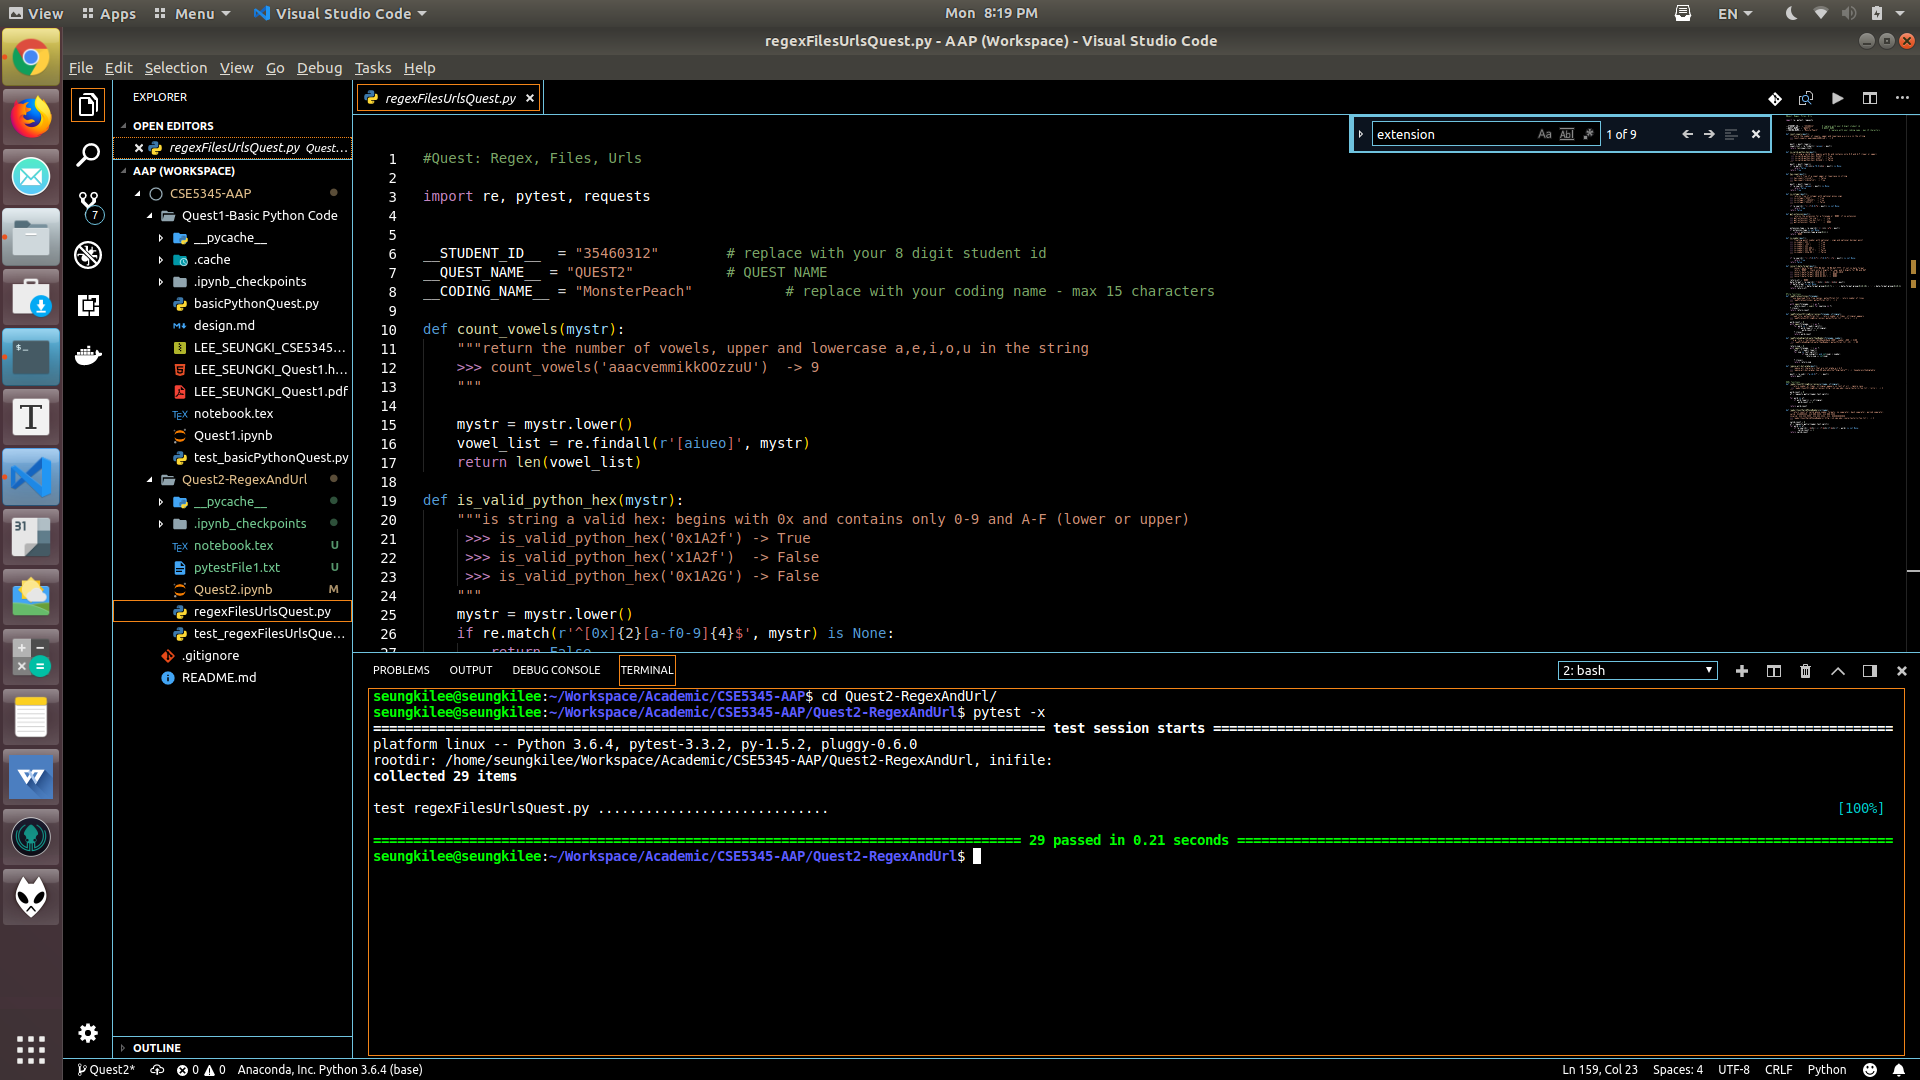
\includegraphics{./pytest2.png}
\caption{Pytest}
\end{figure}


    % Add a bibliography block to the postdoc
    
    
    
    \end{document}
